\documentclass[./main.tex]{subfiles}

\begin{document}
\section{Introduction}
\begin{figure}[htbp]
    \centering
    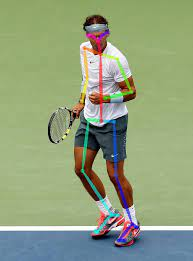
\includegraphics[height = 6 cm]{./entities/pose_estimation_example_img.jpg}
    \caption{Example of 2D single-person articulated human pose \cite{pose_estimation_example}}
    \label{fig:pose_estimation_example_fig}
\end{figure}
% Real-world applications
\noindent It is common knowledge, that the real-world use of artificial intelligence and machine learning is growing rapidly. With this growth the need for accurate computer vision models is also increasing. One usage of computer vision is \textit{human pose estimation}, where a machine learning model is used for estimating the pose of one, or multiple, humans in images or videos. These models have many real-world applications, such as motion analysis, augmented reality and virtual reality \cite{survey_2}.
\\
\\
% Describing pose estimation
There are different types of human pose estimations, where one of the most common ones is the \textit{articulated} human pose estimation, which is done by estimating the location of various keypoints of the human bodies in an input. The methods within human pose estimation can further be split into $2D$ human pose estimation and $3D$ human pose estimation, which describes the amount of dimensions in the estimations. An example of a $2$D articulated human pose of a single person is visualized in Figure \ref{fig:pose_estimation_example_fig}.
\\
\\
% Describing XAI and motivation
As the complexity of machine learning models have increased, the models have started to work more and more as a "black box", where it can be difficult to understand how the models work and why they work as they do. This can often be a problem, especially in cases where the output of the model can result in a life or death situation of a human. For that reason, understanding how a model works can be very important - this is what is called \textit{explainable AI} (\textit{XAI}). Selvaraju \textit{et al.} \cite{Selvaraju} argues that there are three cases for using explainable AI: $(1)$ an understanding of the model can help us improve the performance of the model $(2)$ an understanding of the model can help us build trust in the model, as we can understand its strenghts and weaknesses, and $(3)$ an understanding of the model can teach humans how to perform better, in cases where the model outperforms humans \cite{Selvaraju}.

\subsection{Related Work}
% Related work
Early human pose estimation methods were based on a classic approach. For instance, Felzenszwalb \textit{et al.} use the Histogram of Oriented Gradient features and Support Vector Machines \cite{Felzenszwalb}. More recent pose estimation methods are instead based on deep learning. Toshev \textit{et al.} introduced \textit{DeepPose}, that uses a cascade of deep neural networks to estimate the location of joints, by starting with an estimation based on the full image, which is then refined using sub-images \cite{DeepPose}. Carreira \textit{et al.} developed a self-correcting deep learning model, that works by progressively changing an initial solution by feeding back error predictions \cite{Carreira}. Newell \textit{et al.} introduced the Stacked hourglass, which works by continuously pooling and upsampling the input data to produce a set of heatmaps, where the maximum activation of each heatmap is the location of the corresponding keypoints \cite{Newell}.
\\
\\
There are also a range of different techniques to explain a developed convolutional neural network. Zeiler \textit{et al.} use deconvolutional layers to visualize what each convolutional layer has learned \cite{Zeiler}. Selvaraju \textit{et al.} use a gradient based technique to explain the important regions in an image for a prediction \cite{Selvaraju}. Simonyan \textit{et al.} finds the notion of the various possible outcomes, by generating images that maximises the corresponding class score, as well as develops a technique that computes a class saliency map, given an image and class \cite{Simonyan}. However, few XAI techniques focusing on human pose estimation have been developed. One of the few techniques is \textit{TransPose} developed by Yang \textit{et al.}, which uses a transformer architecture and low-level convolutional blocks to explain what dependencies the location of the predicted keypoint rely on \cite{TransPose}.

\subsection{Problem Statement}
% Problem statement/thesis goals
The goal of this thesis is thus to select and develop a model for $2$D human pose estimation, to interpretate the developed model, as well as use the obtained knowledge about the model to modify and improve the model. We will not be aiming for a very accurate initial model, as we will be focusing on interpretating the model instead. For the model of choice for human pose estimation, we will be using the Stacked hourglass by Newell \textit{et al.} \cite{Newell}. We have decided to make this choice, as the Stacked hourglass is an architecture that has shown state-of-the-art results. At the same time the architecture of the network is similar to the architecture of autoencoders, making the model useful for encoding the data into a lower dimension, which can be useful when we will be doing the interpretation of the model. Our technique for explaining of the network will differ from the techniques explained previously. Instead, we will be looking and analyzing the features of some of the major parts of the Stacked hourglass to get an understanding of the model. Thus, we will not be looking at the minor parts of the Stacked hourglass, such as each convolutional layer like Zeiler \textit{et al.} does \cite{Zeiler}, as our model simply is to deep, making it difficult to figure out what role each part plays.

\subsection{Reading Guide}
% Structure of thesis
In the remainder of this thesis, Section \ref{sec:theory} introduces the basic machine learning theory and Section \ref{sec:algorithms} introduces the most important algortihms used throughout the thesis. In Section \ref{sec:dataset} the used dataset and its preprocessing is described. We then describe our development of a model and its respective results in Section \ref{experiement}, which is then explored and interpreted in Section \ref{sec:XAI}. In Section \ref{sec:improving}, we then use our knowledge of the model to improve the performance of it. We then discuss our approach and results in Section \ref{sec:discussion}. Lastly, we conclude our results in Section \ref{sec:conclusion}.

\end{document}